\documentclass{article}

\usepackage{fancyhdr}
\usepackage{extramarks}
\usepackage{amsmath}
\usepackage{amsthm}
\usepackage{amsfonts}
\usepackage{tikz}
\usepackage{graphicx} %插入图片的宏包
\usepackage{float} %设置图片浮动位置的宏包
\usepackage{pythonhighlight}
% \usepackage{subfigure} %插入多图时用子图显示的宏包
% \usepackage[plain]{algorithm}
% \usepackage{algpseudocode}

% \usetikzlibrary{automata,positioning}

%
% Basic Document Settings
%

\topmargin=-0.45in
\evensidemargin=0in
\oddsidemargin=0in
\textwidth=6.5in
\textheight=9.0in
\headsep=0.25in

\linespread{1.1}

\pagestyle{fancy}
\lhead{\hmwkAuthorName}
\chead{\hmwkClass\ : \hmwkTitle}
\rhead{\firstxmark}
\lfoot{\lastxmark}
\cfoot{\thepage}

\renewcommand\headrulewidth{0.4pt}
\renewcommand\footrulewidth{0.4pt}

\setlength\parindent{0pt}


%代码格式设置



%
% Create Problem Sections
%

\newcommand{\enterProblemHeader}[1]{
    \nobreak\extramarks{}{Problem \arabic{#1} continued on next page\ldots}\nobreak{}
    \nobreak\extramarks{Problem \arabic{#1} (continued)}{Problem \arabic{#1} continued on next page\ldots}\nobreak{}
}

\newcommand{\exitProblemHeader}[1]{
    \nobreak\extramarks{Problem \arabic{#1} (continued)}{Problem \arabic{#1} continued on next page\ldots}\nobreak{}
    \stepcounter{#1}
    \nobreak\extramarks{Problem \arabic{#1}}{}\nobreak{}
}

\setcounter{secnumdepth}{0}
\newcounter{partCounter}
\newcounter{homeworkProblemCounter}
\setcounter{homeworkProblemCounter}{1}
\nobreak\extramarks{Problem \arabic{homeworkProblemCounter}}{}\nobreak{}

%
% Homework Problem Environment
%
% This environment takes an optional argument. When given, it will adjust the
% problem counter. This is useful for when the problems given for your
% assignment aren't sequential. See the last 3 problems of this template for an
% example.
%
\newenvironment{homeworkProblem}[1][-1]{
    \ifnum#1>0
        \setcounter{homeworkProblemCounter}{#1}
    \fi
    \section{Problem \arabic{homeworkProblemCounter}}
    \setcounter{partCounter}{1}
    \enterProblemHeader{homeworkProblemCounter}
}{
    \exitProblemHeader{homeworkProblemCounter}
}

%
% Homework Details
%   - Title
%   - Due date
%   - Class
%   - Section/Time
%   - Instructor
%   - Author
%

\newcommand{\hmwkTitle}{Quiz\ \#13}
\newcommand{\hmwkDueDate}{Jan 30th, 2019}
\newcommand{\hmwkClass}{Complex Networks}
\newcommand{\hmwkClassTime}{Section A}
% \newcommand{\hmwkClassInstructor}{Professor Isaac Newton}
\newcommand{\hmwkAuthorName}{\textbf{RUOPENG XU} }
\newcommand{\hmwkAuthorNum}{\textbf{18M38179} }

%
% Title Page
%

\title{
    \vspace{2in}
    \textmd{\textbf{\hmwkClass:\ \hmwkTitle}}\\
    \normalsize\vspace{0.1in}\small{Due\ on\ \hmwkDueDate\ }\\
    % \vspace{0.1in}\large{\textit{\hmwkClassInstructor\ \hmwkClassTime}}
    \vspace{3in}
}

\author{\hmwkAuthorName\\ \hmwkAuthorNum}
\date{}

\renewcommand{\part}[1]{\textbf{\large Part \Alph{partCounter}}\stepcounter{partCounter}\\}

%
% Various Helper Commands
%

% Useful for algorithms
\newcommand{\alg}[1]{\textsc{\bfseries \footnotesize #1}}

% For derivatives
\newcommand{\deriv}[1]{\frac{\mathrm{d}}{\mathrm{d}x} (#1)}

% For partial derivatives
\newcommand{\pderiv}[2]{\frac{\partial}{\partial #1} (#2)}

% Integral dx
\newcommand{\dx}{\mathrm{d}x}

% Alias for the Solution section header
\newcommand{\solution}{\textbf{\large Solution}}

% Probability commands: Expectation, Variance, Covariance, Bias
\newcommand{\E}{\mathrm{E}}
\newcommand{\Var}{\mathrm{Var}}
\newcommand{\Cov}{\mathrm{Cov}}
\newcommand{\Bias}{\mathrm{Bias}}

\begin{document}

\maketitle

\pagebreak

\begin{homeworkProblem}
    % questions
Do simulations with same parameters (number of nodes, beta, gamma, percentage infected) but with different network structures such as:\\
1. complete graph (clique)\\
2. star graph\\
3. cycle graph\\
4. barbell graph\\
5. lollipop graph\\
% 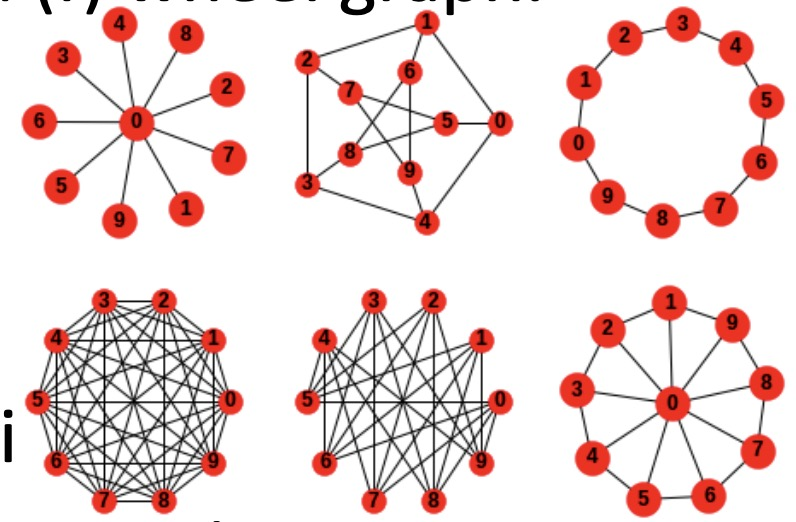
\includegraphics[scale=0.3]{quiz6_1.jpg}

\subsection*{Answer 1}


\begin{python}
!pip install -q ndlib
!pip install -q bokeh

import networkx as nx
import matplotlib.pyplot as plt
import numpy as np
import ndlib.models.epidemics.SIRModel as sir



# Network Definition
g1 = nx.complete_graph(1000)
g2 = nx.star_graph(999)
g3 = nx.cycle_graph(1000)
g4 = nx.barbell_graph(499, 2)
g5 = nx.lollipop_graph(998,2)


# Model Selection
model1 = sir.SIRModel(g1)
model2 = sir.SIRModel(g2)
model3 = sir.SIRModel(g3)
model4 = sir.SIRModel(g4)
model5 = sir.SIRModel(g5)


import ndlib.models.ModelConfig as mc

# Model Configuration
config = mc.Configuration()
config.add_model_parameter('beta', 0.001)
config.add_model_parameter('gamma', 0.01)
config.add_model_parameter("percentage_infected", 0.05)
model1.set_initial_status(config)
model2.set_initial_status(config)
model3.set_initial_status(config)
model4.set_initial_status(config)
model5.set_initial_status(config)


# Simulation
iterations1 = model1.iteration_bunch(200)
trends1 = model1.build_trends(iterations1)

iterations2 = model2.iteration_bunch(200)
trends2 = model2.build_trends(iterations2)

iterations3 = model3.iteration_bunch(200)
trends3 = model3.build_trends(iterations3)

iterations4 = model4.iteration_bunch(200)
trends4 = model4.build_trends(iterations4)

iterations5 = model5.iteration_bunch(200)
trends5 = model5.build_trends(iterations5)

# Visualization
from bokeh.io import output_notebook, show
output_notebook() # there will be no output without this
from ndlib.viz.bokeh.DiffusionTrend import DiffusionTrend

from ndlib.viz.bokeh.DiffusionPrevalence import DiffusionPrevalence


print("complete graph\n", nx.info(g1))
# Diffusion trend
viz1 = DiffusionTrend(model1, trends1)
p1 = viz1.plot(width=400, height=400)
show(p1)

# Prevalence plot
viz1 = DiffusionPrevalence(model1, trends1)
p1 = viz1.plot(width=400, height=400)
show(p1)



print("star graph\n", nx.info(g2))
viz2 = DiffusionTrend(model2, trends2)
p2 = viz2.plot(width=400, height=400)
show(p2)

viz2 = DiffusionPrevalence(model2, trends2)
p2 = viz2.plot(width=400, height=400)
show(p2)


print("cycle graph\n", nx.info(g3))
viz3 = DiffusionTrend(model3, trends3)
p3 = viz3.plot(width=400, height=400)
show(p3)

viz3 = DiffusionPrevalence(model3, trends3)
p3 = viz3.plot(width=400, height=400)
show(p3)


print("barbell graph\n", nx.info(g4))
viz4 = DiffusionTrend(model4, trends4)
p4 = viz4.plot(width=400, height=400)
show(p4)

viz4 = DiffusionPrevalence(model4, trends4)
p4 = viz4.plot(width=400, height=400)
show(p4)



print("lollipop\n", nx.info(g5))
viz5 = DiffusionTrend(model5, trends5)
p5 = viz5.plot(width=400, height=400)
show(p5)

viz5 = DiffusionPrevalence(model5, trends5)
p5 = viz5.plot(width=400, height=400)
show(p5)

## Multiple plot
#from ndlib.viz.bokeh.MultiPlot import MultiPlot
#vm = MultiPlot()
#vm.add_plot(p)
#vm.add_plot(p2)
#m = vm.plot()
#show(m)
\end{python}

The result is:\\
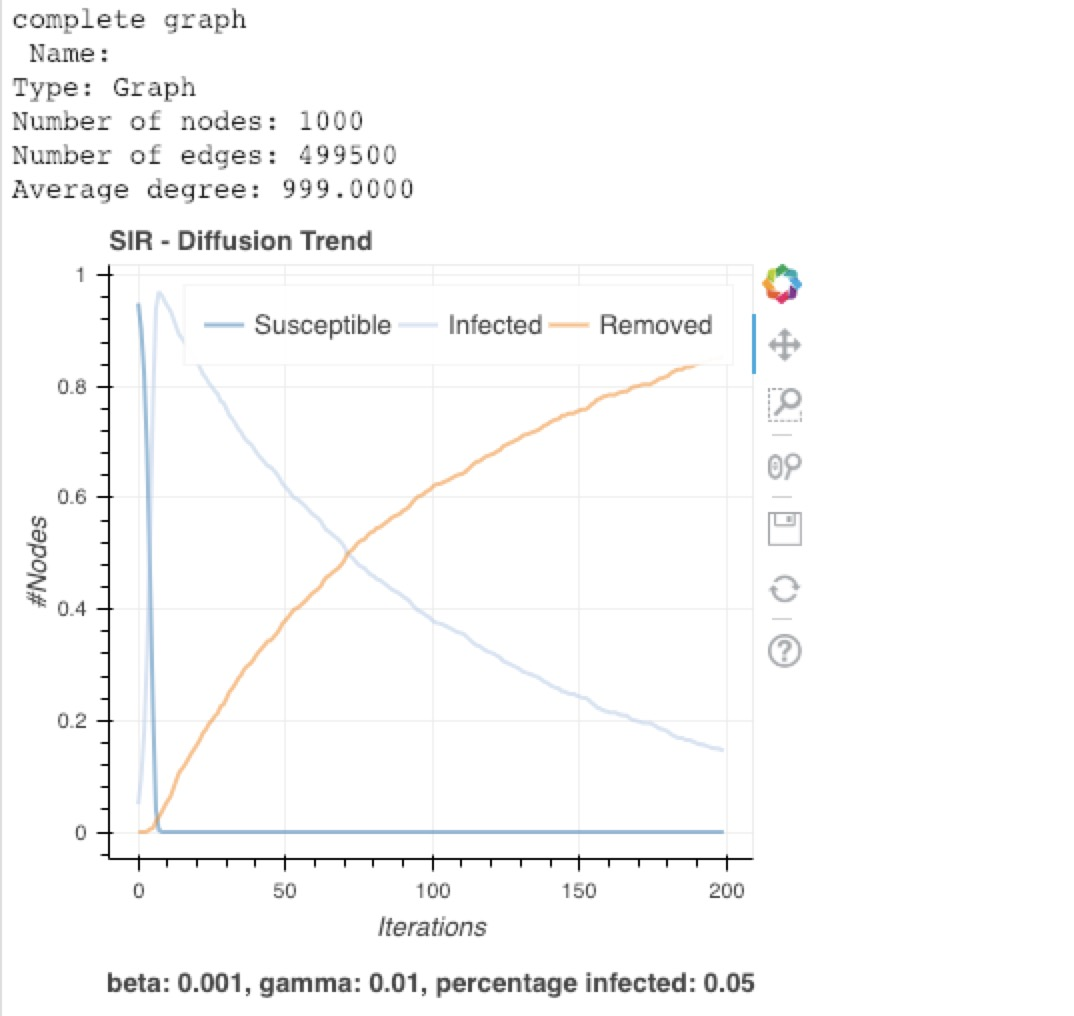
\includegraphics[scale=0.2]{quiz13_1.jpg}
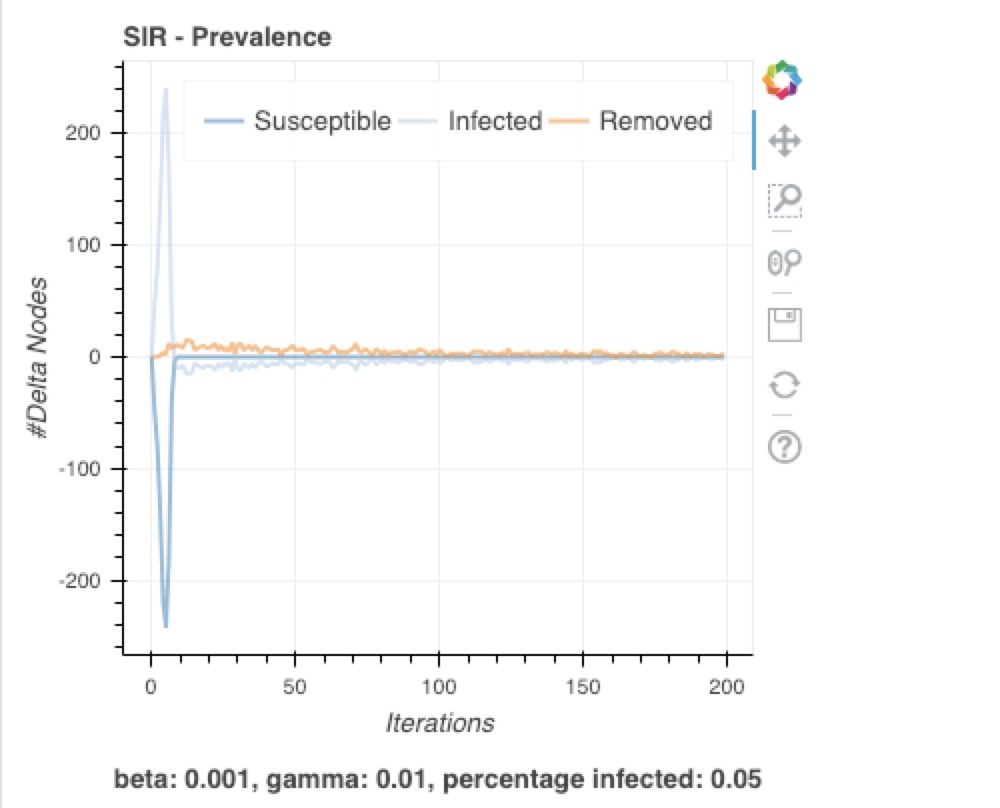
\includegraphics[scale=0.2]{quiz13_2.jpg}\\
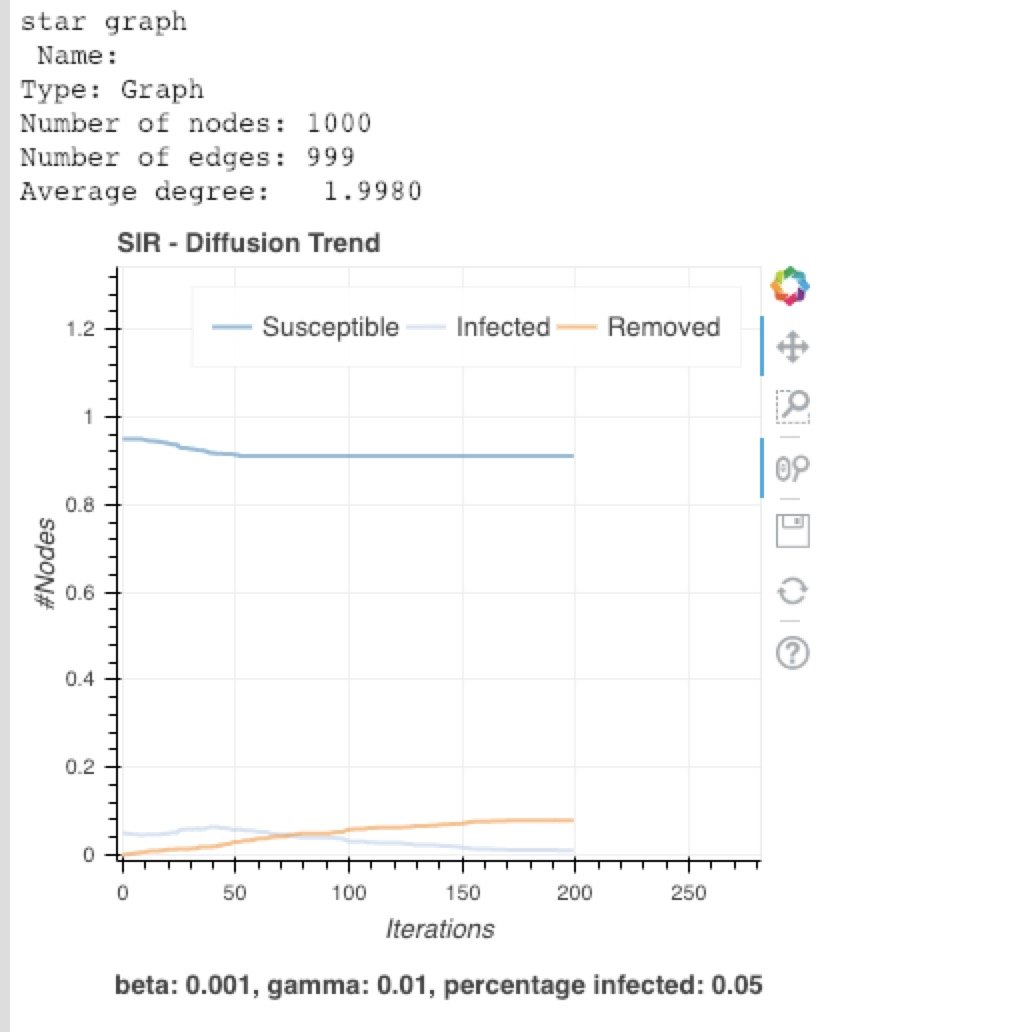
\includegraphics[scale=0.2]{quiz13_3.jpg}
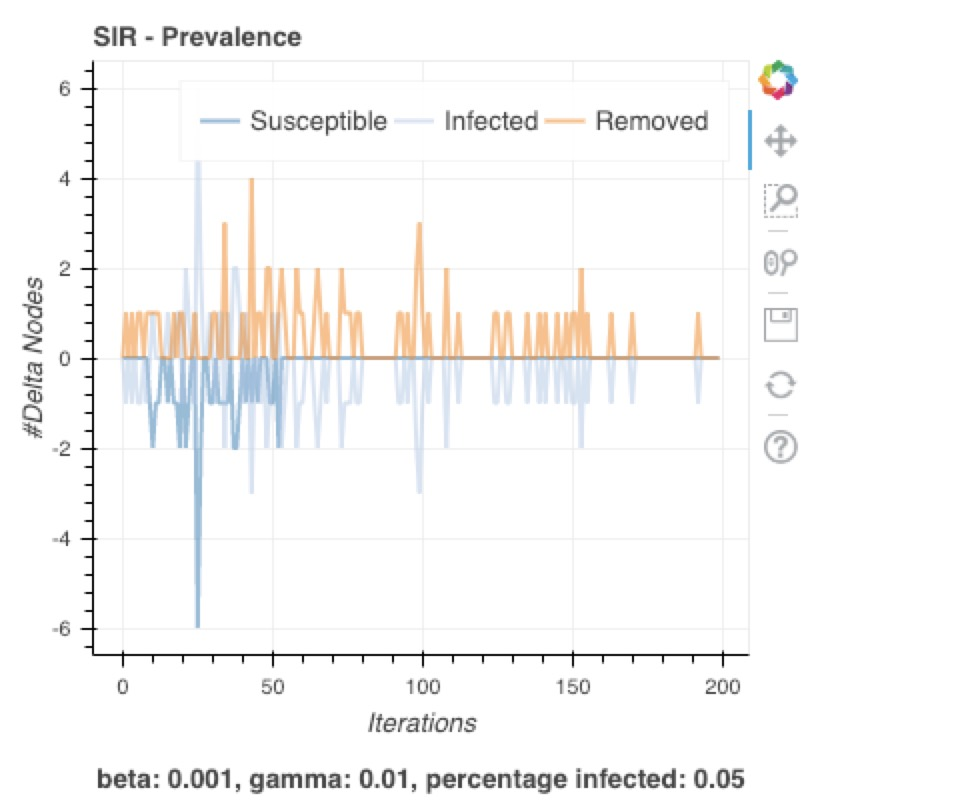
\includegraphics[scale=0.2]{quiz13_4.jpg}\\
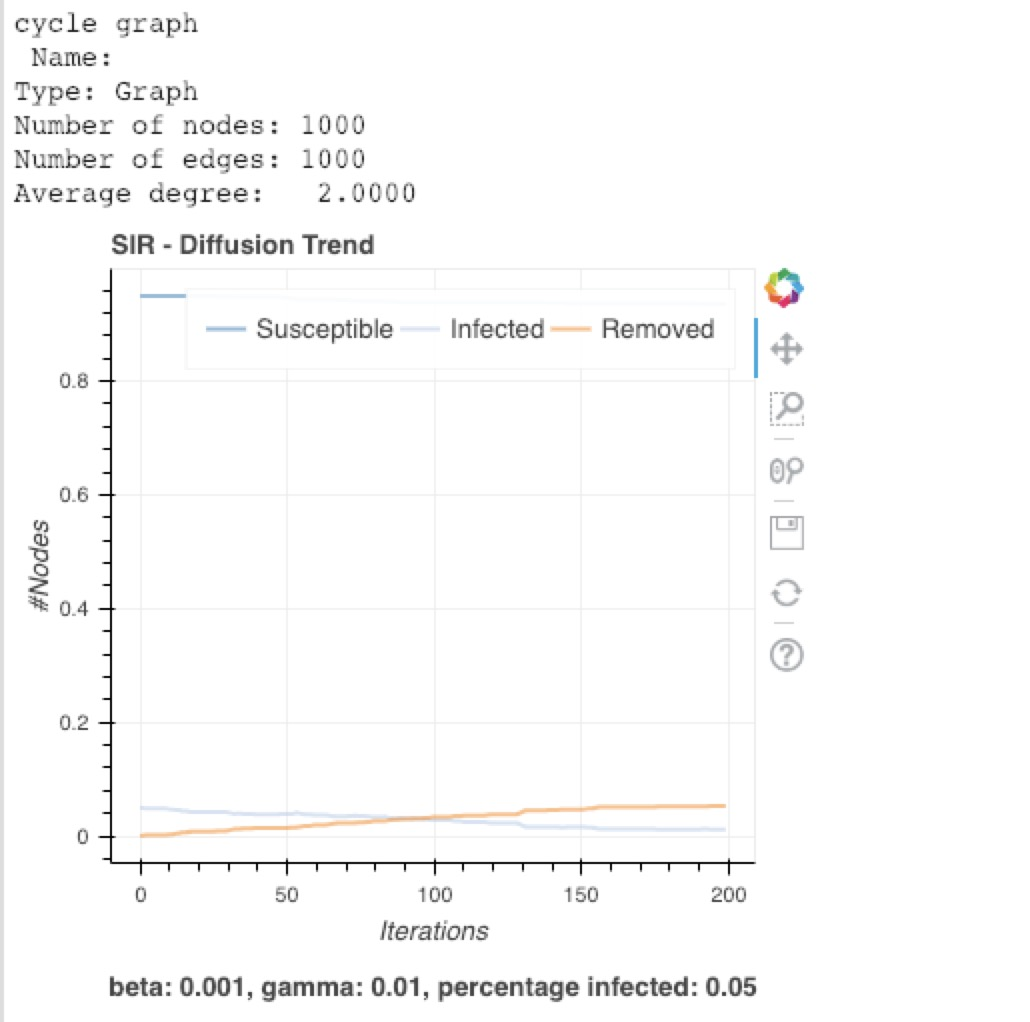
\includegraphics[scale=0.2]{quiz13_5.jpg}
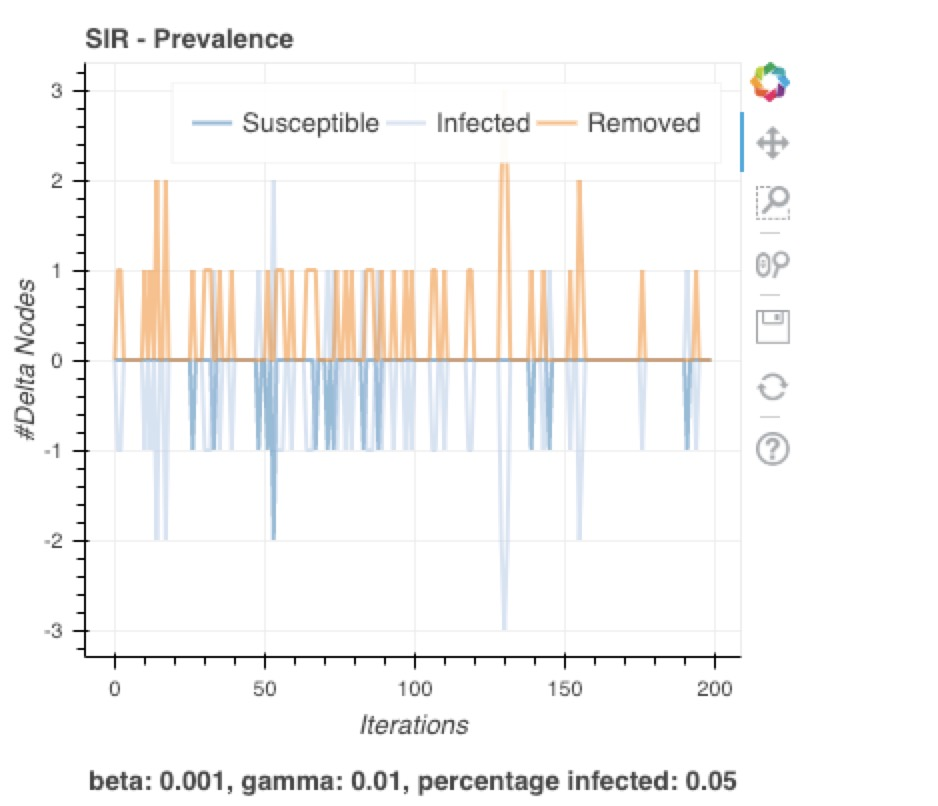
\includegraphics[scale=0.2]{quiz13_6.jpg}\\
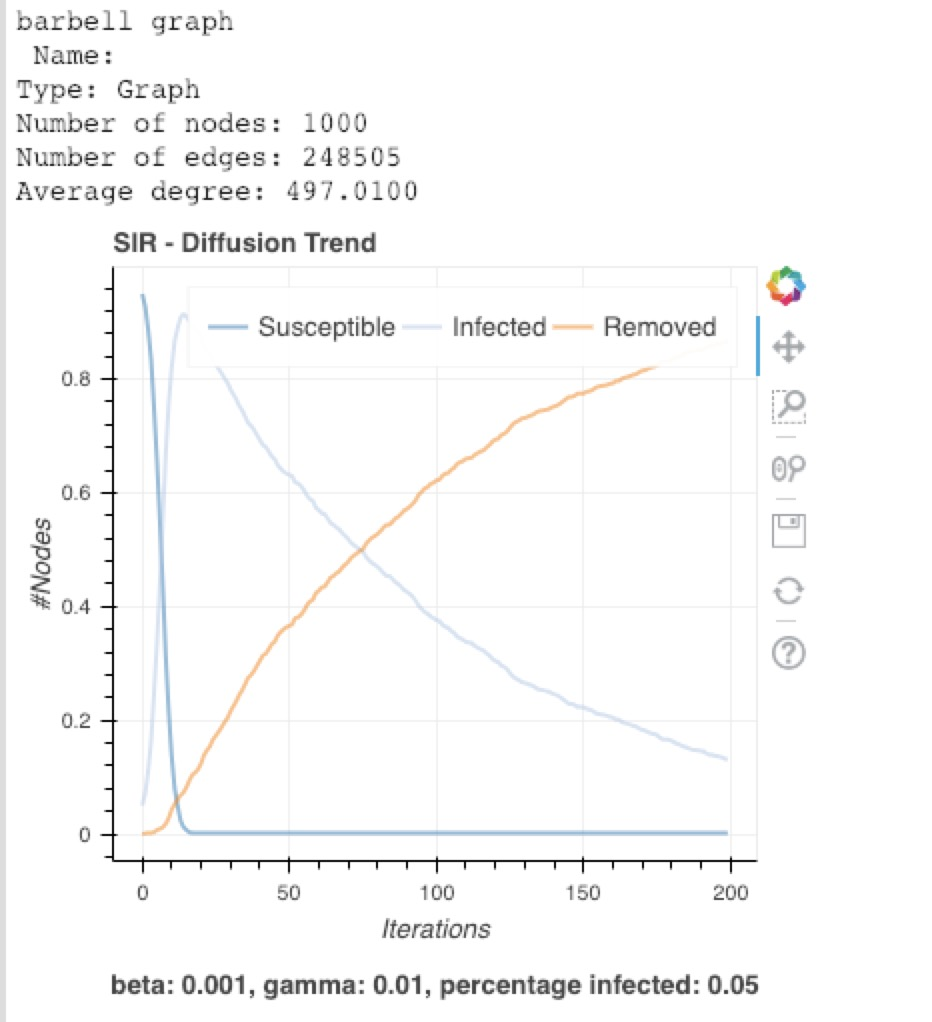
\includegraphics[scale=0.2]{quiz13_7.jpg}
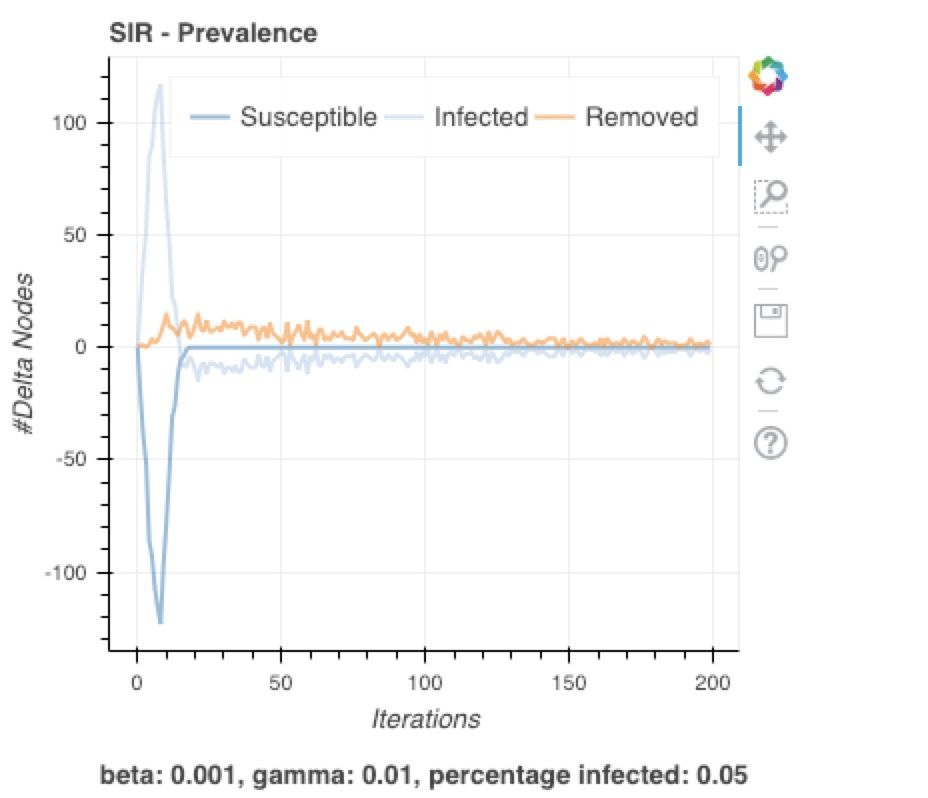
\includegraphics[scale=0.2]{quiz13_8.jpg}\\
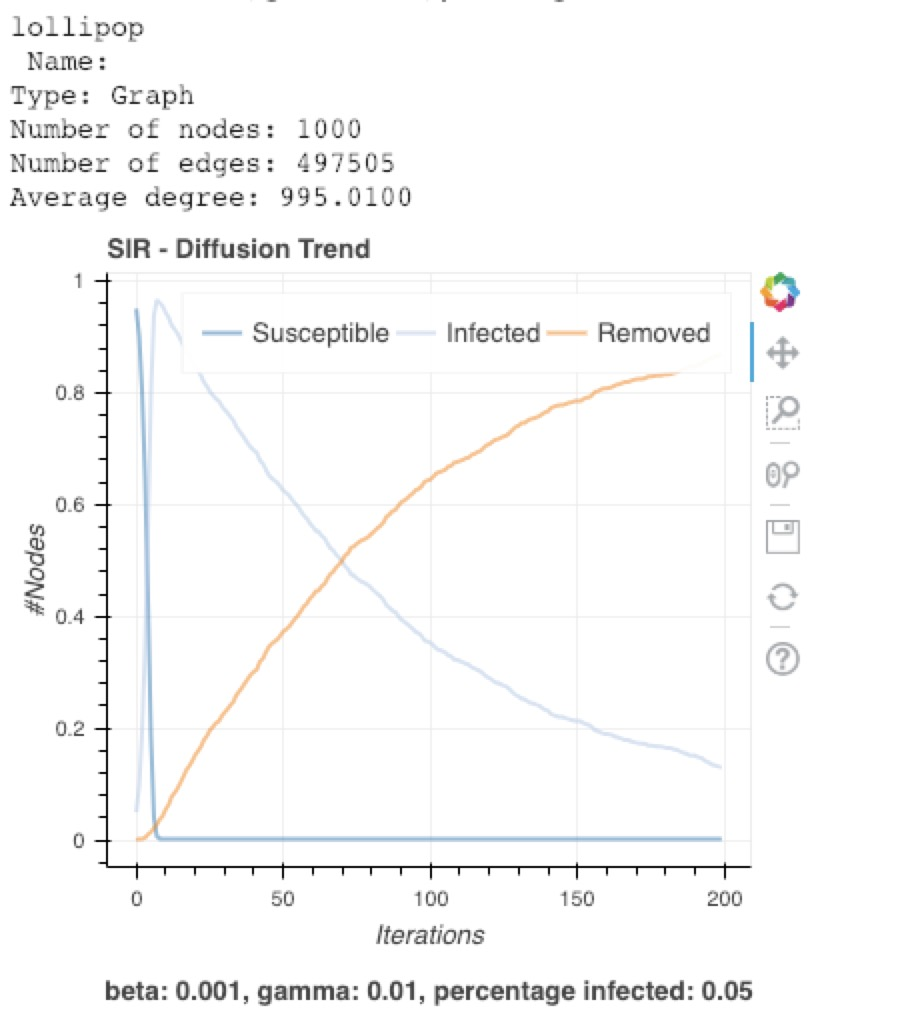
\includegraphics[scale=0.2]{quiz13_9.jpg}
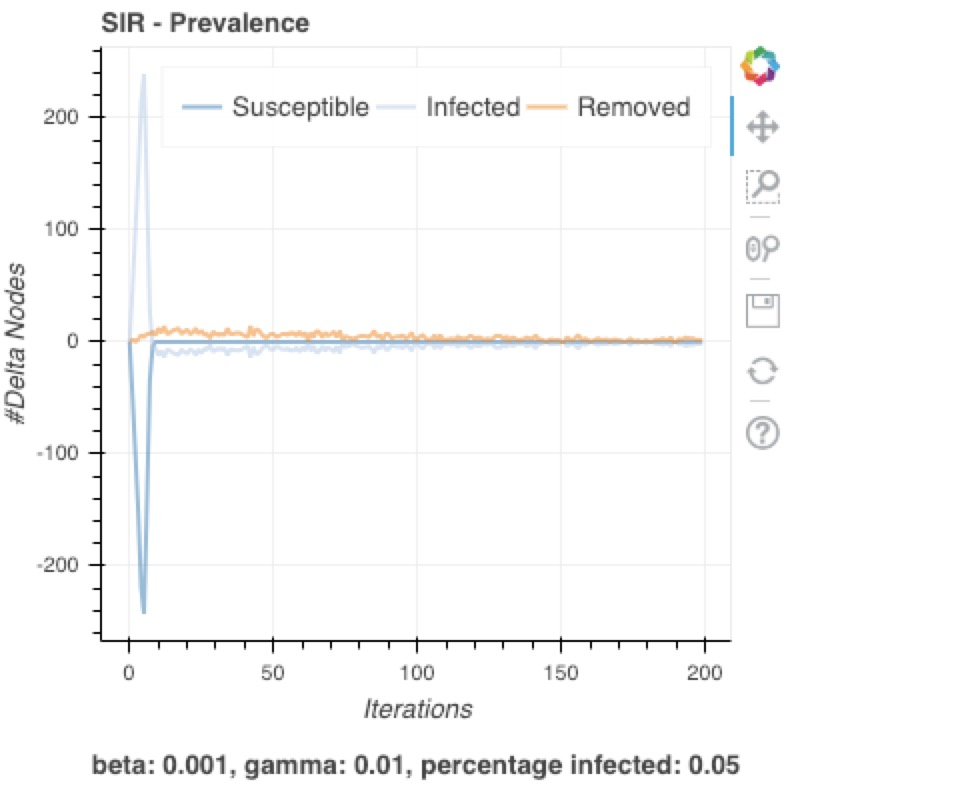
\includegraphics[scale=0.2]{quiz13_10.jpg}\\



\end{homeworkProblem}
\pagebreak

\begin{homeworkProblem}
Show an example of Diffusion Trend which is quite different from that of Erdos‐Renyi network (together with used network structure).

\subsection*{Answer 2}
From the images above, we can find that the Diffusion Trend of star graph and cycle graph is quite different from Erdos-Renyi network. From the images we can see that the infected people increase much slower than the infected in Erdos-Renyi. In 200 interations, there are less than 200 infected in 1000 people, which is because the edge between nodes are less so that the disease is difficult for spreading.


\end{homeworkProblem}
\pagebreak


\end{document}
%
% Non sequential homework problems
%

% Jump to problem 18
